\documentclass[10pt,a4paper]{article}
\usepackage[utf8]{inputenc}
\usepackage[T1]{fontenc}
\usepackage{lmodern}
\usepackage{microtype}
\renewcommand{\familydefault}{\sfdefault}
\usepackage[a4paper,margin=9.5mm,top=7mm,bottom=7mm]{geometry}
\usepackage{xcolor}
\usepackage{amssymb}
\usepackage{graphicx}
\usepackage{tikz}
\usepackage{tcolorbox}
\tcbuselibrary{skins}
\usepackage{enumitem}
\usepackage[hidelinks]{hyperref}

% ── Palette Premium : Bleu Glacier, Bleu Nuit, Teal & Or Discret ──
\definecolor{marginBlue}{HTML}{DCE9F5}     % Marges extérieures bleu clair
\definecolor{marginBorder}{HTML}{B5CBE0}   % Filet architectural extérieur
\definecolor{headerBg}{HTML}{EDF4FA}       % En-tête bleu glacier doux
\definecolor{headerBorder}{HTML}{C5D7E8}   % Séparateur en-tête
\definecolor{sidebarBg}{HTML}{F2F6FA}      % Colonne latérale ardoise claire
\definecolor{sidebarLine}{HTML}{D4E1ED}    % Ligne séparatrice colonne
\definecolor{primaryDark}{HTML}{0F2438}    % Bleu nuit profond
\definecolor{sectionNavy}{HTML}{1A3F63}    % Bleu Oxford structurant
\definecolor{accentTeal}{HTML}{0F6B63}     % Teal éditorial (cohérent portfolio)
\definecolor{bodyText}{HTML}{1E293B}       % Texte ardoise foncé lisible
\definecolor{mutedSlate}{HTML}{52606D}     % Métadonnées et contextes
\definecolor{subtleRule}{HTML}{CBD8E4}     % Filets fins de projet
\definecolor{goldAccent}{HTML}{9A5B13}     % Ambre doré pour distinction

\newcommand{\editorialfont}{\fontfamily{lmr}\selectfont\itshape}

\hypersetup{
  pdfauthor={KOA Marie Gervais Nelly},
  pdftitle={KOA Marie Gervais Nelly | Ingénieur IA \& Architecte Data}
}

\pagestyle{empty}
\setlength{\parindent}{0pt}
\setlength{\parskip}{0pt}
\hyphenpenalty=10000
\exhyphenpenalty=10000

\newcommand{\mainSecTitle}[1]{%
  \vspace{11pt}%
  {\fontsize{11.0}{13.0}\selectfont\textbf{\color{sectionNavy}\MakeUppercase{#1}}}\\[2.5pt]%
  {\color{accentTeal}\rule{19mm}{1.2pt}\color{subtleRule}\rule{\dimexpr\linewidth-19mm\relax}{0.6pt}}\\[6pt]%
}

\newcommand{\sideSecTitle}[1]{%
  \vspace{11pt}%
  {\fontsize{10.3}{12.4}\selectfont\textbf{\color{sectionNavy}\MakeUppercase{#1}}}\\[2.5pt]%
  {\color{accentTeal}\rule{14mm}{1.1pt}\color{subtleRule}\rule{\dimexpr\linewidth-14mm\relax}{0.55pt}}\\[5.5pt]%
}

\newcommand{\devbadge}{%
  \tikz[baseline=-0.6pt]{\node[draw=accentTeal,fill=white,rounded corners=1.2pt,inner xsep=1.5pt,inner ysep=0.8pt,font=\fontsize{4.9}{5.2}\selectfont\bfseries\color{accentTeal}]{DEV};}%
}

\begin{document}

% ── FOND BLEU CLAIR DANS LES MARGES + FEUILLE BLANCHE + SIDEBAR PLEINE HAUTEUR ──
\begin{tikzpicture}[remember picture, overlay]
  \fill[marginBlue] (current page.south west) rectangle (current page.north east);
  \fill[white] ([xshift=4.8mm,yshift=4.8mm]current page.south west) rectangle ([xshift=-4.8mm,yshift=-4.8mm]current page.north east);
  \fill[sidebarBg] ([xshift=4.8mm,yshift=4.8mm]current page.south west) rectangle ([xshift=72.2mm,yshift=-43.0mm]current page.north west);
  \draw[sidebarLine, line width=0.6pt] ([xshift=72.2mm,yshift=4.8mm]current page.south west) -- ([xshift=72.2mm,yshift=-43.0mm]current page.north west);
  \fill[headerBg] ([xshift=4.8mm,yshift=-43.0mm]current page.north west) rectangle ([xshift=-4.8mm,yshift=-4.8mm]current page.north east);
  \draw[headerBorder, line width=0.7pt] ([xshift=4.8mm,yshift=-43.0mm]current page.north west) -- ([xshift=-4.8mm,yshift=-43.0mm]current page.north east);
  \fill[primaryDark] ([xshift=4.8mm,yshift=-4.8mm]current page.north west) rectangle ([xshift=-65mm,yshift=-6.4mm]current page.north east);
  \fill[accentTeal] ([xshift=-65mm,yshift=-4.8mm]current page.north east) rectangle ([xshift=-4.8mm,yshift=-6.4mm]current page.north east);
  \draw[marginBorder, line width=0.8pt] ([xshift=4.8mm,yshift=4.8mm]current page.south west) rectangle ([xshift=-4.8mm,yshift=-4.8mm]current page.north east);
\end{tikzpicture}

% ── EN-TÊTE STRUCTURÉ : PORTRAIT + IDENTITÉ + COORDONNÉES ALIGNÉES ──
\vspace*{0.8mm}
\noindent\begin{minipage}[c]{0.135\textwidth}
  \centering
  \begin{tikzpicture}
    \clip (0,0) circle (1.16cm);
    \node at (0,0) {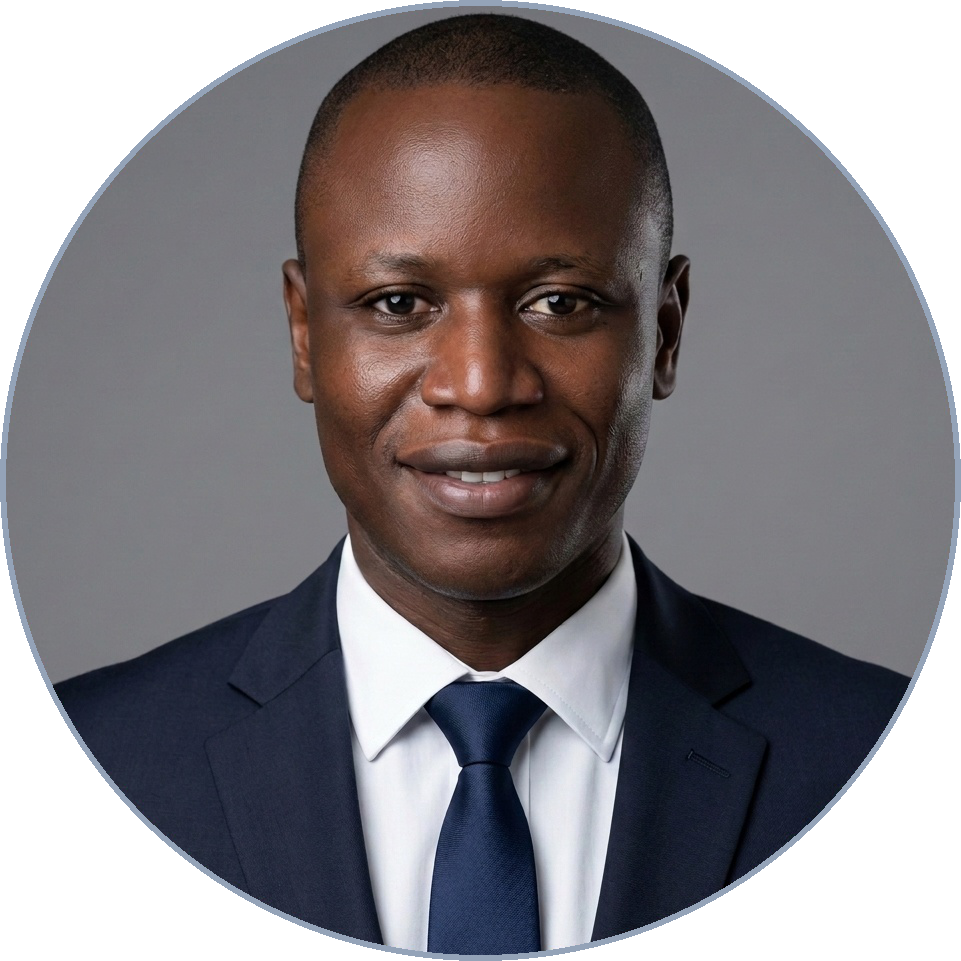
\includegraphics[width=2.34cm]{profile_headshot_clean.png}};
    \draw[white, line width=1.8pt] (0,0) circle (1.15cm);
    \draw[headerBorder, line width=0.9pt] (0,0) circle (1.16cm);
  \end{tikzpicture}
\end{minipage}%
\hspace{0.022\textwidth}%
\begin{minipage}[c]{0.843\textwidth}
  \raggedright
  {\fontsize{18.0}{20.2}\selectfont\textbf{\color{primaryDark}KOA}\hspace{6pt}{\fontsize{16.5}{20.2}\selectfont\color{sectionNavy}Marie Gervais Nelly}}\\[2.5pt]
  {\fontsize{10.9}{13.0}\selectfont\textbf{\color{sectionNavy}Ingénieur IA \& Architecte Data}}%
  \hspace{5pt}{\color{mutedSlate}\textbar}\hspace{5pt}%
  {\editorialfont\fontsize{10.1}{12.5}\selectfont\color{accentTeal}Systèmes RAG, Orchestration Agentique \& Données}\\[4.5pt]
  {\fontsize{8.4}{10.5}\selectfont\color{bodyText}
  \raisebox{-1.0pt}{
\includegraphics[height=7.0pt]{icons/icon_location.png}}\hspace{3pt}Douala / Ngaoundéré, Cameroun%
  \quad{\color{marginBorder}\textbar}\quad
  \raisebox{-1.0pt}{
\includegraphics[height=6.8pt]{icons/icon_phone.png}}\hspace{3pt}\href{tel:+237695353402}{\color{bodyText}+237 695 35 34 02}%
  \quad{\color{marginBorder}\textbar}\quad
  \raisebox{-1.0pt}{
\includegraphics[height=6.7pt]{icons/icon_email.png}}\hspace{3pt}\href{mailto:contact@archicam-ai.com}{\textbf{\color{primaryDark}contact@archicam-ai.com}}
  }\\[3.2pt]
  {\color{headerBorder}\rule{\linewidth}{0.5pt}}\\[3.5pt]
  {\fontsize{8.3}{10.5}\selectfont
  \begin{tabular}{@{}p{0.50\linewidth}p{0.46\linewidth}@{}}
    \raisebox{-1.0pt}{
\includegraphics[height=6.9pt]{icons/icon_globe.png}}\hspace{3pt}\href{https://portfolio-gervais.vercel.app}{\textbf{\color{primaryDark}portfolio-gervais.vercel.app}} &
    \raisebox{-1.0pt}{
\includegraphics[height=6.9pt]{icons/icon_github.png}}\hspace{3pt}\href{https://github.com/gervais-afk}{\color{bodyText}github.com/gervais-afk} \\[2.2pt]
    \raisebox{-1.0pt}{
\includegraphics[height=6.9pt]{icons/icon_linkedin.png}}\hspace{3pt}\href{https://linkedin.com/in/marie-gervais-koa}{\color{bodyText}linkedin.com/in/marie-gervais-koa} &
    \devbadge\hspace{3pt}\href{https://dev.to/gervais_marie}{\color{bodyText}dev.to/gervais\_marie}
  \end{tabular}}
\end{minipage}

\vspace{7.5mm}

% ── DEUX COLONNES : SIDEBAR GAUCHE (31%) & CORPS PRINCIPAL DROIT (69%) ──
\noindent\begin{minipage}[t]{0.310\textwidth}
  \raggedright
  \vspace{0pt}
  \sideSecTitle{Compétences techniques}
  \textbf{\color{sectionNavy}\fontsize{10.0}{12.2}\selectfont IA \& Recherche}\\[2.2pt]
  {\fontsize{9.6}{13.0}\selectfont\color{bodyText}PyTorch, RAG / recherche hybride, Adversarial ML (FGSM), Antigravity, Claude, Codex, Motion design avec IA}
\vspace{10pt}

  \textbf{\color{sectionNavy}\fontsize{10.0}{12.2}\selectfont Ingénierie \& Agents}\\[2.2pt]
  {\fontsize{9.6}{13.0}\selectfont\color{bodyText}Python, TypeScript, FastAPI, Genkit, CrewAI, MCP/FastMCP, Docker, pytest, Zod}
\vspace{10pt}

  \textbf{\color{sectionNavy}\fontsize{10.0}{12.2}\selectfont Données \& MLOps}\\[2.2pt]
  {\fontsize{9.6}{13.0}\selectfont\color{bodyText}SQL, PostgreSQL/pgvector, SQLite, Neo4j/Cypher, Cassandra, MongoDB, OLAP, scikit-learn, Optuna, MLflow, nbformat, SHA-256}

  \vspace{6pt}
  \sideSecTitle{Formation}
  \textbf{\color{primaryDark}\fontsize{9.9}{12.5}\selectfont Master Professionnel \textperiodcentered{} Intelligence Artificielle Appliquée}\\[1.8pt]
  {\fontsize{8.9}{11.2}\selectfont\color{mutedSlate}Déc. 2025--2027 \textperiodcentered{} en cours}\\[2.5pt]
  {\fontsize{9.5}{12.9}\selectfont\color{bodyText}Univ. de Ngaoundéré \textperiodcentered{} Cours : ML, Big Data, Vision, NoSQL, Ontologies, Cybersécurité, Droit \& Éthique IA, Prompt Engineering, Comm. des organisations, Entrepreneuriat.}
\vspace{11pt}

  \textbf{\color{primaryDark}\fontsize{9.9}{12.5}\selectfont Licence \& BTS \textperiodcentered{} Génie Civil, option bâtiment}\\[1.8pt]
  {\fontsize{8.9}{11.2}\selectfont\color{mutedSlate}2015--2016}\\[2.5pt]
  {\fontsize{9.5}{12.9}\selectfont\color{bodyText}ISTDI / IUC Douala \textperiodcentered{} Cameroun \textperiodcentered{} Cours : Résistance des matériaux, calcul de structures, métrés et gestion de chantier.}

  \vspace{6pt}
  \sideSecTitle{Langues}
  {\fontsize{9.6}{13.1}\selectfont\color{bodyText}Français natif \textperiodcentered{} Anglais intermédiaire : lecture et compréhension orale ; expression orale simple.}

  \vspace{6pt}
  \sideSecTitle{Distinction}
  {\fontsize{9.6}{13.1}\selectfont\color{bodyText}\textcolor{goldAccent}{$\bigstar$}\ Attestation d’Excellence \& Intégrité \textperiodcentered{} CCAA, 2023.}
\end{minipage}%
\hspace{0.042\textwidth}%
\begin{minipage}[t]{0.648\textwidth}
  \raggedright
  \vspace{0pt}
  \mainSecTitle{PROFIL}
  \begin{tcolorbox}[enhanced, frame hidden, colback=sidebarBg,
    borderline west={2.2pt}{0pt}{accentTeal},
    left=8pt, right=7pt, top=7pt, bottom=7pt, boxsep=0pt, arc=1.5pt]
    \raggedright
    {\fontsize{10.0}{13.8}\selectfont\color{bodyText}Ingénieur IA \& Architecte Data, titulaire d’un Master professionnel en Intelligence Artificielle Appliquée : je conçois des systèmes de recherche documentaire (RAG, graphes), d’orchestration agentique et d’automatisation Data, avec une rigueur issue du génie civil et de la sûreté aéroportuaire.}
  \end{tcolorbox}

  \vspace{3pt}
  \mainSecTitle{Projets IA \& Data}
  \begin{tcolorbox}[enhanced, frame hidden, interior hidden,
    borderline west={1.8pt}{0pt}{accentTeal},
    left=8pt, right=0pt, top=1.5pt, bottom=1.5pt, boxsep=0pt]
    \raggedright
    {\fontsize{11.2}{13.4}\selectfont\textbf{\color{primaryDark}K1-MathInfo}}\\[2pt]
    {\fontsize{9.1}{12.1}\selectfont\color{mutedSlate}Projet Master pour le département de mathématiques et informatique de l’Université de Ngaoundéré (en binôme ; contribution personnelle transversale).}\\[3pt]
    \begin{itemize}[leftmargin=10pt,label={\color{accentTeal}\tiny$\blacksquare$},itemsep=3.2pt,topsep=1.5pt,parsep=0pt]
    \item {\fontsize{9.9}{13.5}\selectfont\color{bodyText}525 travaux (2010--2026) : recherche hybride avec références et abstention ; recommandations explicables par Jaccard pondéré.}
    \item {\fontsize{9.9}{13.5}\selectfont\color{bodyText}Entrepôt en étoile à six dimensions pour l’OLAP.}
    \end{itemize}
  \end{tcolorbox}
\vspace{10pt}
  \begin{tcolorbox}[enhanced, frame hidden, interior hidden,
    borderline west={1.0pt}{0pt}{subtleRule},
    left=8pt, right=0pt, top=1.5pt, bottom=1.5pt, boxsep=0pt]
    \raggedright
    {\fontsize{11.2}{13.4}\selectfont\textbf{\color{primaryDark}Archi Cam AI}}\\[2pt]
    {\fontsize{9.1}{12.1}\selectfont\color{mutedSlate}Projet personnel \textperiodcentered{} IA appliquée au BTP \textperiodcentered{} Développé dans le cadre de Google Applied Africa AI Lab.}\\[3pt]
    \begin{itemize}[leftmargin=10pt,label={\color{accentTeal}\tiny$\blacksquare$},itemsep=3.2pt,topsep=1.5pt,parsep=0pt]
    \item {\fontsize{9.9}{13.5}\selectfont\color{bodyText}Chiffrage, métrés, DQE et calculs métier : développement d’outils en lien direct avec ma formation en génie civil.}
    \end{itemize}
  \end{tcolorbox}
\vspace{10pt}
  \begin{tcolorbox}[enhanced, frame hidden, interior hidden,
    borderline west={1.0pt}{0pt}{subtleRule},
    left=8pt, right=0pt, top=1.5pt, bottom=1.5pt, boxsep=0pt]
    \raggedright
    {\fontsize{11.2}{13.4}\selectfont\textbf{\color{primaryDark}Dataset Automator}}\\[2pt]
    {\fontsize{9.1}{12.1}\selectfont\color{mutedSlate}Prototype individuel développé dans le cadre du Google Cloud \#AllThingsAgentic Hackathon.}\\[3pt]
    \begin{itemize}[leftmargin=10pt,label={\color{accentTeal}\tiny$\blacksquare$},itemsep=3.2pt,topsep=1.5pt,parsep=0pt]
    \item {\fontsize{9.9}{13.5}\selectfont\color{bodyText}Automatisation du profilage, du nettoyage de fichiers CSV et de la comparaison de modèles tabulaires sur un flux reproductible.}
    \item {\fontsize{9.9}{13.5}\selectfont\color{bodyText}Application de règles métier, suivi des expériences et génération de notebooks Jupyter documentés et prêts à l’exécution.}
    \end{itemize}
  \end{tcolorbox}

  \vspace{3pt}
  \mainSecTitle{Expérience professionnelle}
  \noindent\begin{tabular*}{\linewidth}{@{}p{0.76\linewidth}@{\extracolsep{\fill}}r@{}}
    \textbf{\color{primaryDark}\fontsize{10.4}{12.8}\selectfont Consultant IA \& Data indépendant} &
    {\fontsize{8.9}{11.0}\selectfont\color{mutedSlate}Mars 2026 -- présent}
  \end{tabular*}\\[2.5pt]
  {\fontsize{9.8}{13.4}\selectfont\color{bodyText}Conception de pipelines IA \& Data et accompagnement technique sur des besoins métier.}
\vspace{10pt}

  \noindent\begin{tabular*}{\linewidth}{@{}p{0.76\linewidth}@{\extracolsep{\fill}}r@{}}
    \textbf{\color{primaryDark}\fontsize{10.4}{12.8}\selectfont Agent puis Chef de Groupe sûreté aéroportuaire (AVSEC) \textperiodcentered{} CCAA} &
    {\fontsize{8.9}{11.0}\selectfont\color{mutedSlate}2018 -- présent}
  \end{tabular*}\\[2.5pt]
  {\fontsize{9.8}{13.4}\selectfont\color{bodyText}Analyse des risques opérationnels, contrôle qualité des équipements de détection, traçabilité et rédaction de rapports d’incidents.}
\end{minipage}

\end{document}
